\subsection{Etude de $f(x)= \frac{e^{x}}{\ln(x)} $}
\begin{exercice}
Soit $f$ la fonction définie par 
$$f(x)= \frac{e^{x}}{\ln(x)} $$
\begin{enumerate}
\item Donner l'ensemble de définition et de dérivation de $f$. 
\item Calculer la dérivée de $f$ en déduire que le signe de $f'$ dépend de celui de $g(x)=\ln(x) - \frac{1}{x}$
\item Donner l'ensemble de définition et de dérivation de $g$ et calculer sa dérivée. 
\item Montrer qu'il existe un unique $\alpha\in ]1,+\infty[$ tel que $f'(x)>0$ sur $]\alpha, +\infty[$ et $f'(x)<0$ sur $]0,\alpha[\cap D_f$. 
\item Donner le tableau de variations complet de $f$. 
\item Donner l'équation de la tangente à la courbe représentative de $f$ en $e$.

\end{enumerate}
\end{exercice}

\begin{correction}
\begin{enumerate}
\item La fonction $\exp$ est définie  et dérivable sur $\R$. La fonction $ \ln$ est définie et dérivable sur $]0,+\infty[$. La fonction inverse est définie et dérivabel sur $\R^*$ et enfin $\ln(x) =0$ si et seulement si $x=1$ donc la fonction $f$ est définie  et dérivable sur $D_f= ]0,1[\cup]1,+\infty[$. 
\item On  a pour tout $x\in D_f$ 
$$f'(x)=\frac{e^x \ln(x)- e^x\frac{1}{x}}{\ln^2(x)} = \frac{e^x}{\log^2(x)} g(x) $$
Comme poru tout $x\in D_f$, $\frac{e^x}{\log^2(x)}\geq 0$, 
 le signe de $f'$ est égal à celui de $g(x)=\ln(x)-\frac{1}{x}$. 
 
 \item $g$ est définie et dérivable sur $]0,+\infty[$ et on a $g'(x)=\frac{1}{x}+\frac{1}{x^2}$ Ainsi $g'(x)$ est positif prou tout $x\in  ]0,+\infty[$. 
 
 \item La fonciton $g$ est strictement croissante. Comme $\lim_{x\tv 
 0} g(x)  = -\infty$ $\lim_{x\tv 
 \infty } g(x)  = \infty$, le théorème de la bijection assure qu'il existe un unique $\alpha \in ]0,+\infty[ $ tel que $g(\alpha) =0$ 
 
 Comme $g(1) = -1 < 0$ et que $g$ est strictement croissante, on a de plus $\alpha>1$ 

 \item 
\begin{center}
\begin{tikzpicture}
\tkzTabInit[espcl=6]{$x$ / 1,Signe de\\$f'(x)$/1, Variations de\\ $f$ / 3}%
{$0$, $1$, $+\infty$}%
\tkzTabLine{,-,h,+, }
\tkzTabVar{+/$0$ , -/$-\infty$,+/$+\infty$ }
   \end{tikzpicture}
\end{center}


\item On a $f'(e) = e^e g(e) = -e^e(1-\frac{1}{e})  =-e^{e}+e^{e-1}$ et $f(e) = e^{e}$
Donc l'équation de la tangente à la courbe représentative de $f$ en $e$ et donnée par 
$$y-e^{e} =(-e^{e}+e^{e-1} )(x-e)$$
\end{enumerate}
\end{correction}